\section{Experimental setup}
 
In order to determine the tire characteristics of the scaled vehicle, a good testbed is necessary. In this section, the experimental setup used to gather the data needed for determining the tire characteristic is discussed. As concluded from the model, the following variables are required to measure the tire characteristics: 
\begin{itemize}
	\item$\bullet$ linear accelerations of the car
    \item$\bullet$ linear and angular velocities of the car
    \item$\bullet$ steering angle of the front wheels
    \item$\bullet$ angular velocities of the wheels
\end{itemize}
The experimental setup consists of a modified scaled RC car with an on board IMU, feedback servo and a tachometer on each wheel. Moreover, a motion capture system, or MoCap, was used to provide millimeter precision localization. The IMU is used to measure the velocities and accelerations of the car. The feedback from the servo is used to determine the steering angle. The tachometers are used to measure the angular velocity of the wheels. The MoCap was used to check and calibrate the signal coming from the IMU. However, the noise on the MoCap location signal, which is amplified by differentiation, made it unfit for this research.

\subsection{Car}
The RC car is a Losi TEN Rally-X. It is a 1:10 scale car with 4WD powered by a 2s 6000 mAh LiPo battery and a 3900 KV Fuze Brushless DC motor. With this battery the car is able drive at speeds between 1.5 and 15 m/s.  To meet the assumptions of the Bicycle model, the suspension of the car was replaced with stiff turnbuckle rods to eliminate the degrees of freedom of roll and pitch. The wheels are custom 3D-printed rims with grip tape applied to simulate tires and fitted with 2 magnets each. When the magnets pass a hall-effect sensor on the car a signal is created of 2 pulses per revolution. The hall-effect sensors and the magnets make up the tachometers of the car. Another set of wheels with space for 24 magnets was created, but due to lack of time, no tests were conducted with these. The IMU was mounted in the center of gravity of the car, preventing angular velocities from influencing the accelerometer. Finally, the standard servomotor was replaced by a robot servomotor, which allowed for reading the angle from the servomotor angle sensor.

\subsubsection{MoCap}
The MoCap is used as a positioning system. A MoCap system cannot be regarded as an on-board sensor, as it requires an area with aligned cameras. However, in this case it is used as a replacement for a GPS sensor. The MoCap system enables us to do testing inside, something which is not possible with a GPS system. Finally, the MoCap system was ready to use and already connected with ROS, using a sampling rate of 120 Hz.

\begin{figure*}
  \centering
    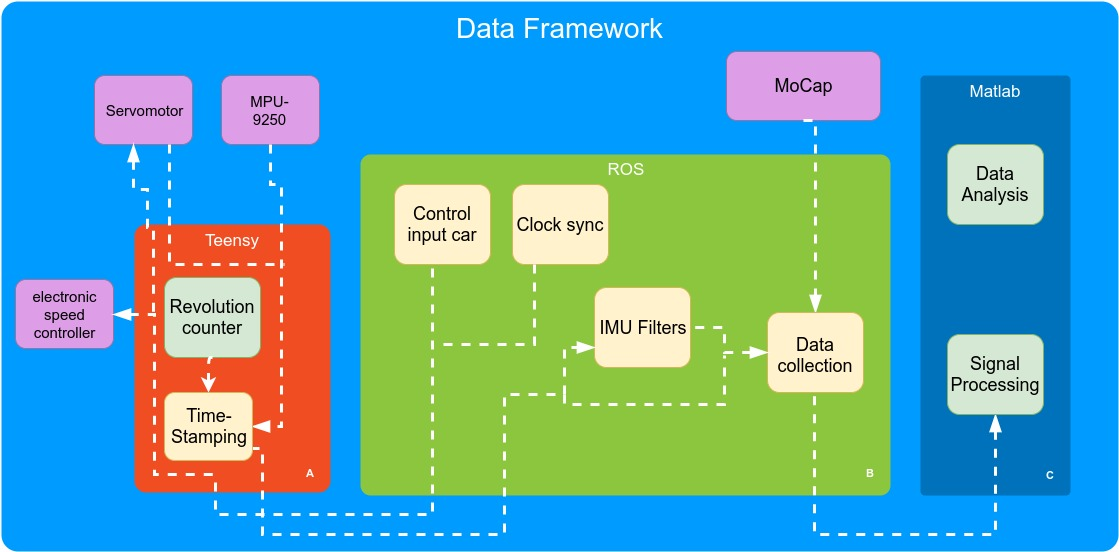
\includegraphics[scale=0.40]{figure/DataFramework__1_.jpg}
  \caption{Data acquisition framework}
  \label{fig:DonutFramework} 
\end{figure*}

\subsection{Data acquisition and processing}
Data acquisition was done using a ROS (Robot Operating System) based system. The sensors were connected to a Teensy 3.6 prototyping board running a custom ROSserial node, connected to a Raspberry Pi 3 model B running ROS. The custom ROSserial node uses an interrupt controlled program to gather sensor data in a fast and accurate way. Moreover, on-board hardware timers were employed as pulse counters for the tachometer-signal.
The MoCap is connected to the system utilizing the labs Wi-Fi network. Further communication was done using a self-written ROS package. After data collection, further processing was done using Matlab. Figure
\ref{fig:DonutFramework} further elaborates the Data acquisition framework.

\subsubsection{ROS}
Implementing ROS on the testbed provided it with some key components needed for accurate testing. Since ROS has already been established as a research and prototyping framework, a lot of packages are already developed for this operating system and are easily available.  One key component is timestamping. To provide usable data, the testbed needs a timestamping method. ROS automatically syncs all the clocks on every device providing a convenient solution to this problem. Furthermore, our testbed contains a simple IMU which does not provide all data that a more advanced IMU might offer, like orientation or sensor fusion between the magnetometer and gyroscope signal. Therefore a complementary filter was used in ROS to generate this data. \cite{IMUfilter}. The complementary filter was chosen for this purpose as its transfer function and implementation is the same as a Kalman filter. However the complementary filter has improved response time. Moreover, the MoCap generated its data already in ROS, which meant combining everything in ROS would be a simplification. Also, ROS offers convenient data recording options called ROSbags, which can be imported into MATLAB for further analysis.

\subsubsection{Sampling}
The sampling rate for our experiments was set at 120 Hz. The MoCap already operated at this sampling rate and to simplify synchronizing our data points one sampling rate was used. Moreover, if all sensors would work on the same sampling rate, this would reduce the hardware requirements on the Teensy and reduce the need for data interpolating. 

Since a lot of noise was apparent on the IMU signal in initial tests, the decision was made to employ the built-in Digital Low Pass Filter (DLPF) on the IMU, to decrease noise and data rate at the same time. However, this would create a delay on our signal. To prevent this delay from becoming significant, a limit of 10ms signal delay was chosen. A 92 Hz DLPF was chosen since it only created a delay of 7.8 ms, but would decrease the data rate significantly without losing data points. To prevent signal aliasing, a sampling rate of 92 Hz or higher is required. Our sampling rate of 120 Hz fills this requirement

% Since the MoCap already delivered her data at a sampling rate of 120 Hz, it was easy to pick this as the target sampling rate for the whole system. Because initial tests showed no accelerations beyond 1.5 g, this would mean the maximum increase of velocity per timestep would be 0.122[m/s]. This was deemed accurate enough for this research. Moreover, testing will also be done at speeds as slow as 1.5[m/s], including accelerating from standstill. With 24 magnets this would result in signals of 127 Hz. If the sampling frequency would be higher than the frequency of wheel pulses, this would generate multiple points with the same distance traveled, as no new pulses from the wheel were encountered in between. This increases signal analysis difficulty requiring further interpolation before analysis can be done. Since the goal was always to use 24 magnets per wheel, this sampling rate was used from the beginning. Moreover, 2 magnets would create a signal with a frequency of only 10.6 Hz. As a sampling frequency of 10 Hz or even lower has a resolution of only 0.1 s, in which a pulse could have been generated at any given time, this was deemed too low so the sampling rate was kept at 120 Hz. Furthermore, the IMU generates data at sampling rates reaching 1000 Hz. Testing showed however, that ROS was only capable of reaching speeds of 300Hz on the Raspberry Pi. Moreover, since a lot of noise was apparent in initial tests, the decision was made to employ the built-in Digital Low Pass Filter(DLPF) to decrease noise and data rate at the same time. However, this would create a delay on our signal. To prevent this delay from becoming significant, a limit of 10ms signal delay was chosen. A 92 Hz DLPF was chosen since it only created a delay of 7.8 ms, but this decreased the data rate significantly without losing data points. To prevent aliasing, a sampling rate of 92 Hz or higher was needed. This made it possible to have all the sensors to work on the same sampling rate to reduce hardware requirements on the Teensy and reduce data interpolating. 

\subsubsection{Experiments}
The experiments can be classified into three groups.

The first set of experiments is carried out in a straight line (longitudinal motion). During these experiments, the car accelerated and braked while driving straight ahead. 

The second set consists of the steady state cornering experiments (lateral motion). Steady state cornering means cornering at a constant longitudinal velocity and constant steering angle. 

Finally, the third set of experiments take both lateral and longitudinal motion into account. Variables of the tests are acceleration/deceleration for longitudinal motion, longitudinal velocity and steering angle for lateral motion, and these three combined for combined motion. The variables were slightly increased in each experiment in order to determine the transition from linear to nonlinear behaviour.

\subsection{Data filter} 	
The experimental data is collected in ROSbags and processed afterwards. This makes it possible to filter the noise from the IMU with a Zero-Phase Low Pass Butterworth Filter. This is a non-causal filter with a phase slope of zero which eliminates any delay that is commonly caused by causal filters. The Low Pass filter is of the 20th order, in order to approach an ideal Brick wall Response, with a cut-off frequency of 5Hz. A Fourier spectrum analysis was done, however the signal from the IMU was indistinguishable from the noise. Therefore, it was reasoned most of the noise would be from vibrations generated by the wheels and at the minimal speed of 1.5 m/s these would rotate at 5.3 Hz. Therefore a "Brick wall" response, as seen in figure (\ref{fig:brickwall}) at 5 Hz was selected. This would cancel out most of the noise, but keeps most of the signal intact. 
	\begin{figure}
	\centering
	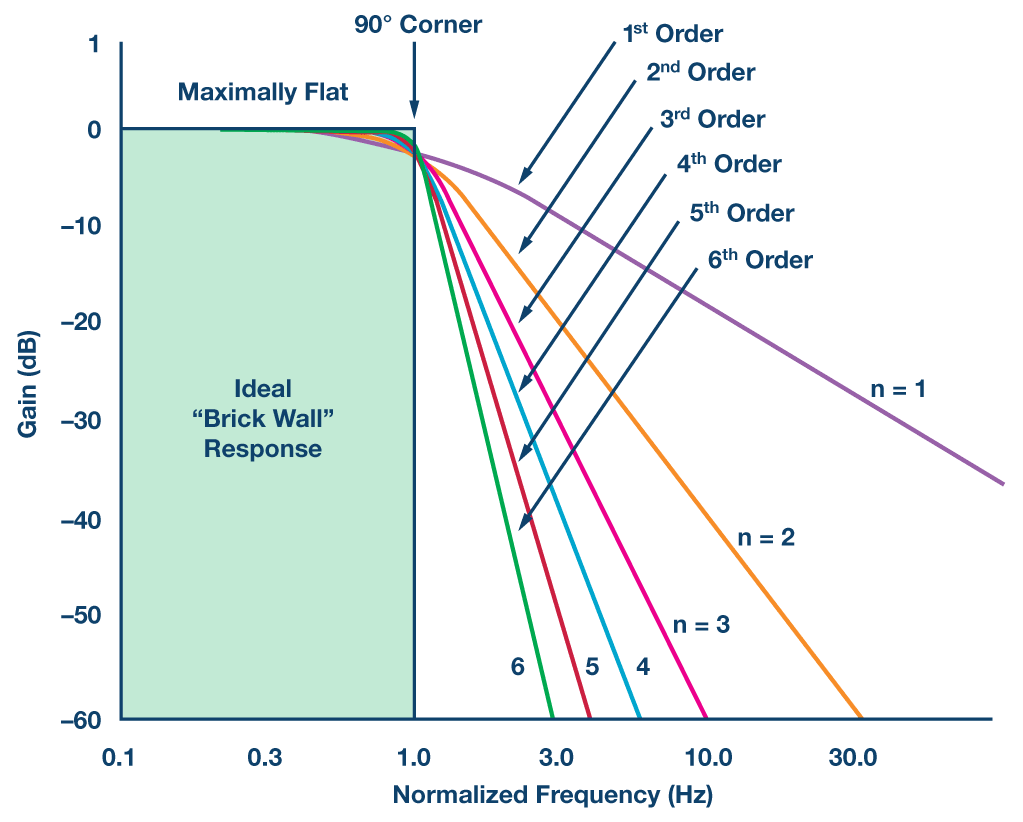
\includegraphics[scale=0.17]{figure/brickwall.png}
	\caption{Brick wall response}
	%\captionsource{Caption}{(http://www.electronics-tutorials.ws/filter/filter_8.html)}
	\label{fig:brickwall}
	\end{figure}





